\documentclass[presentation, bigger]{beamer}
\usepackage{etex}
\usepackage[utf8]{inputenc}
\usepackage[T1]{fontenc}
\usepackage{fixltx2e}
\usepackage{graphicx}
\usepackage{longtable}
\usepackage{float}
\usepackage{wrapfig}
\usepackage[normalem]{ulem}
\usepackage{textcomp}
\usepackage{marvosym}
\usepackage{wasysym}
\usepackage{latexsym}
\usepackage{amssymb}
\usepackage{amstext}
\usepackage{hyperref}
\usepackage{url}
\usepackage{multimedia}
\usepackage[dutch]{babel}
\usepackage[font=scriptsize,labelfont=bf]{caption}
\setbeamertemplate{caption}[numbered]
% \usepackage{pgfpages}
% \setbeameroption{show notes on second screen=right}
\setbeamercolor*{block body example}{bg= blue!5}
\usepackage{tikz}
%% 
% \usepackage{enumitem}
\usepackage{booktabs}

%% code
\usepackage{listings}
\usepackage{color}
\usepackage{verbatim}

\definecolor{codegreen}{rgb}{0,0.6,0}
\definecolor{codegray}{rgb}{0.5,0.5,0.5}
\definecolor{codepurple}{rgb}{0.58,0,0.82}
\definecolor{backcolour}{rgb}{0.95,0.95,0.92}

\lstdefinestyle{mystyle}{
  backgroundcolor=\color{backcolour},   
  commentstyle=\color{codegreen},
  keywordstyle=\color{magenta},
  numberstyle=\tiny\color{codegray},
  stringstyle=\color{codepurple},
  basicstyle=\footnotesize,
  breakatwhitespace=false,         
  breaklines=true,                 
  captionpos=b,                    
  keepspaces=true,                 
  numbers=left,                    
  numbersep=5pt,                  
  showspaces=false,                
  showstringspaces=false,
  showtabs=false,                  
  tabsize=2
}

\tolerance=1000
\usetheme{kuleuven}
\useinnertheme{rectangles}
\graphicspath{{graphics/}}
\usepackage[style=authoryear,hyperref,backref,square,natbib,ibidtracker=false]{biblatex}
\bibliography{bibliography}

\usepackage{graphicx}
\usetheme{default}
\author{Ward Schodts, Xavier Goás Aguililla}
\date{Dinsdag 5 mei 2015}
\title{Internet of Things code deployment metrics}
\newcommand{\aheader}[2]{\action<#1-|alert@#1>{#2}}
% first argument: slide number to appear from, second argument: content of header 
\newcommand{\hiddencell}[2]{\action<#1->{#2}}
% first argument: slide number to appear from, second argument: content of cell

\DeclareBibliographyCategory{papers}


\begin{document}

\maketitle
\begin{frame}[noframenumbering]{Outline}
  \tableofcontents
  \note{3 grote luiken\\
  }
\end{frame}



\section{Inleiding}
\begin{frame}{Wireless sensor networks}

  \begin{figure}
    \fbox{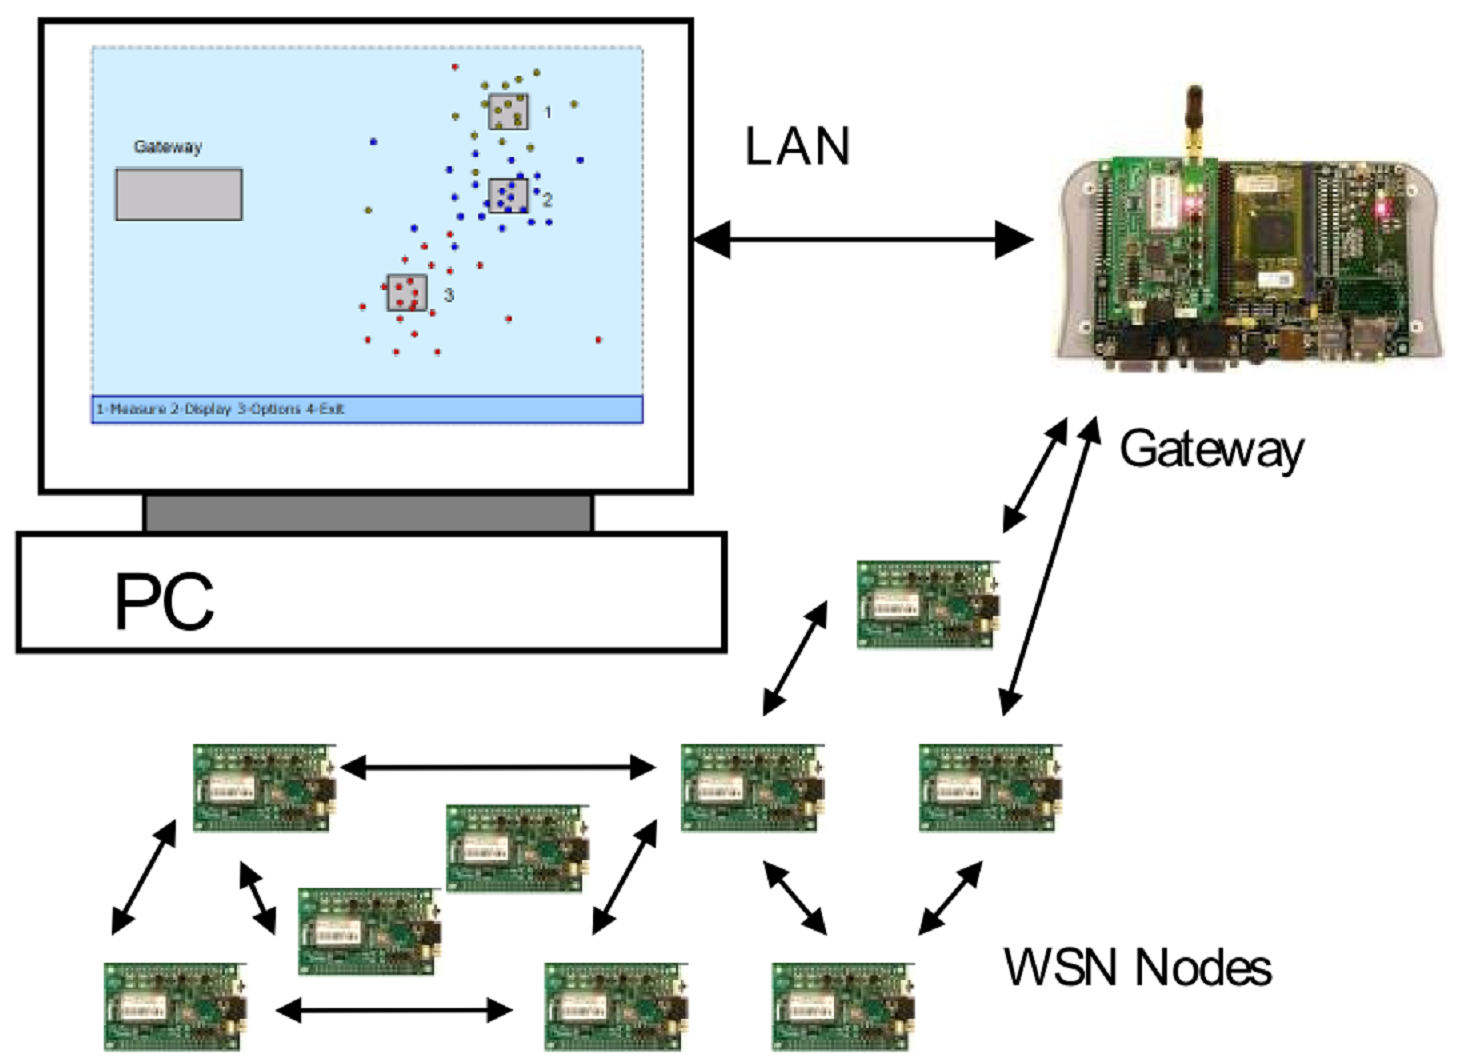
\includegraphics[width=0.82\textwidth,keepaspectration=true]{intro/overview.png}}
    \caption{Een wireless sensor network}
  \end{figure}
  \note{
    \begin{itemize}
    \item heel veel, sensoren enkele gateways
    \item netwerk bestaande uit sensoren
    \item ad-hoc netwerk technieken, geen bestaande!
    \item geen routing door 1 centrale unit
    \item communiceren via elkaar

    \end{itemize}
  }
\end{frame}

% \begin{frame}{Wireless sensor networks}
%   \begin{figure}
%     \fbox{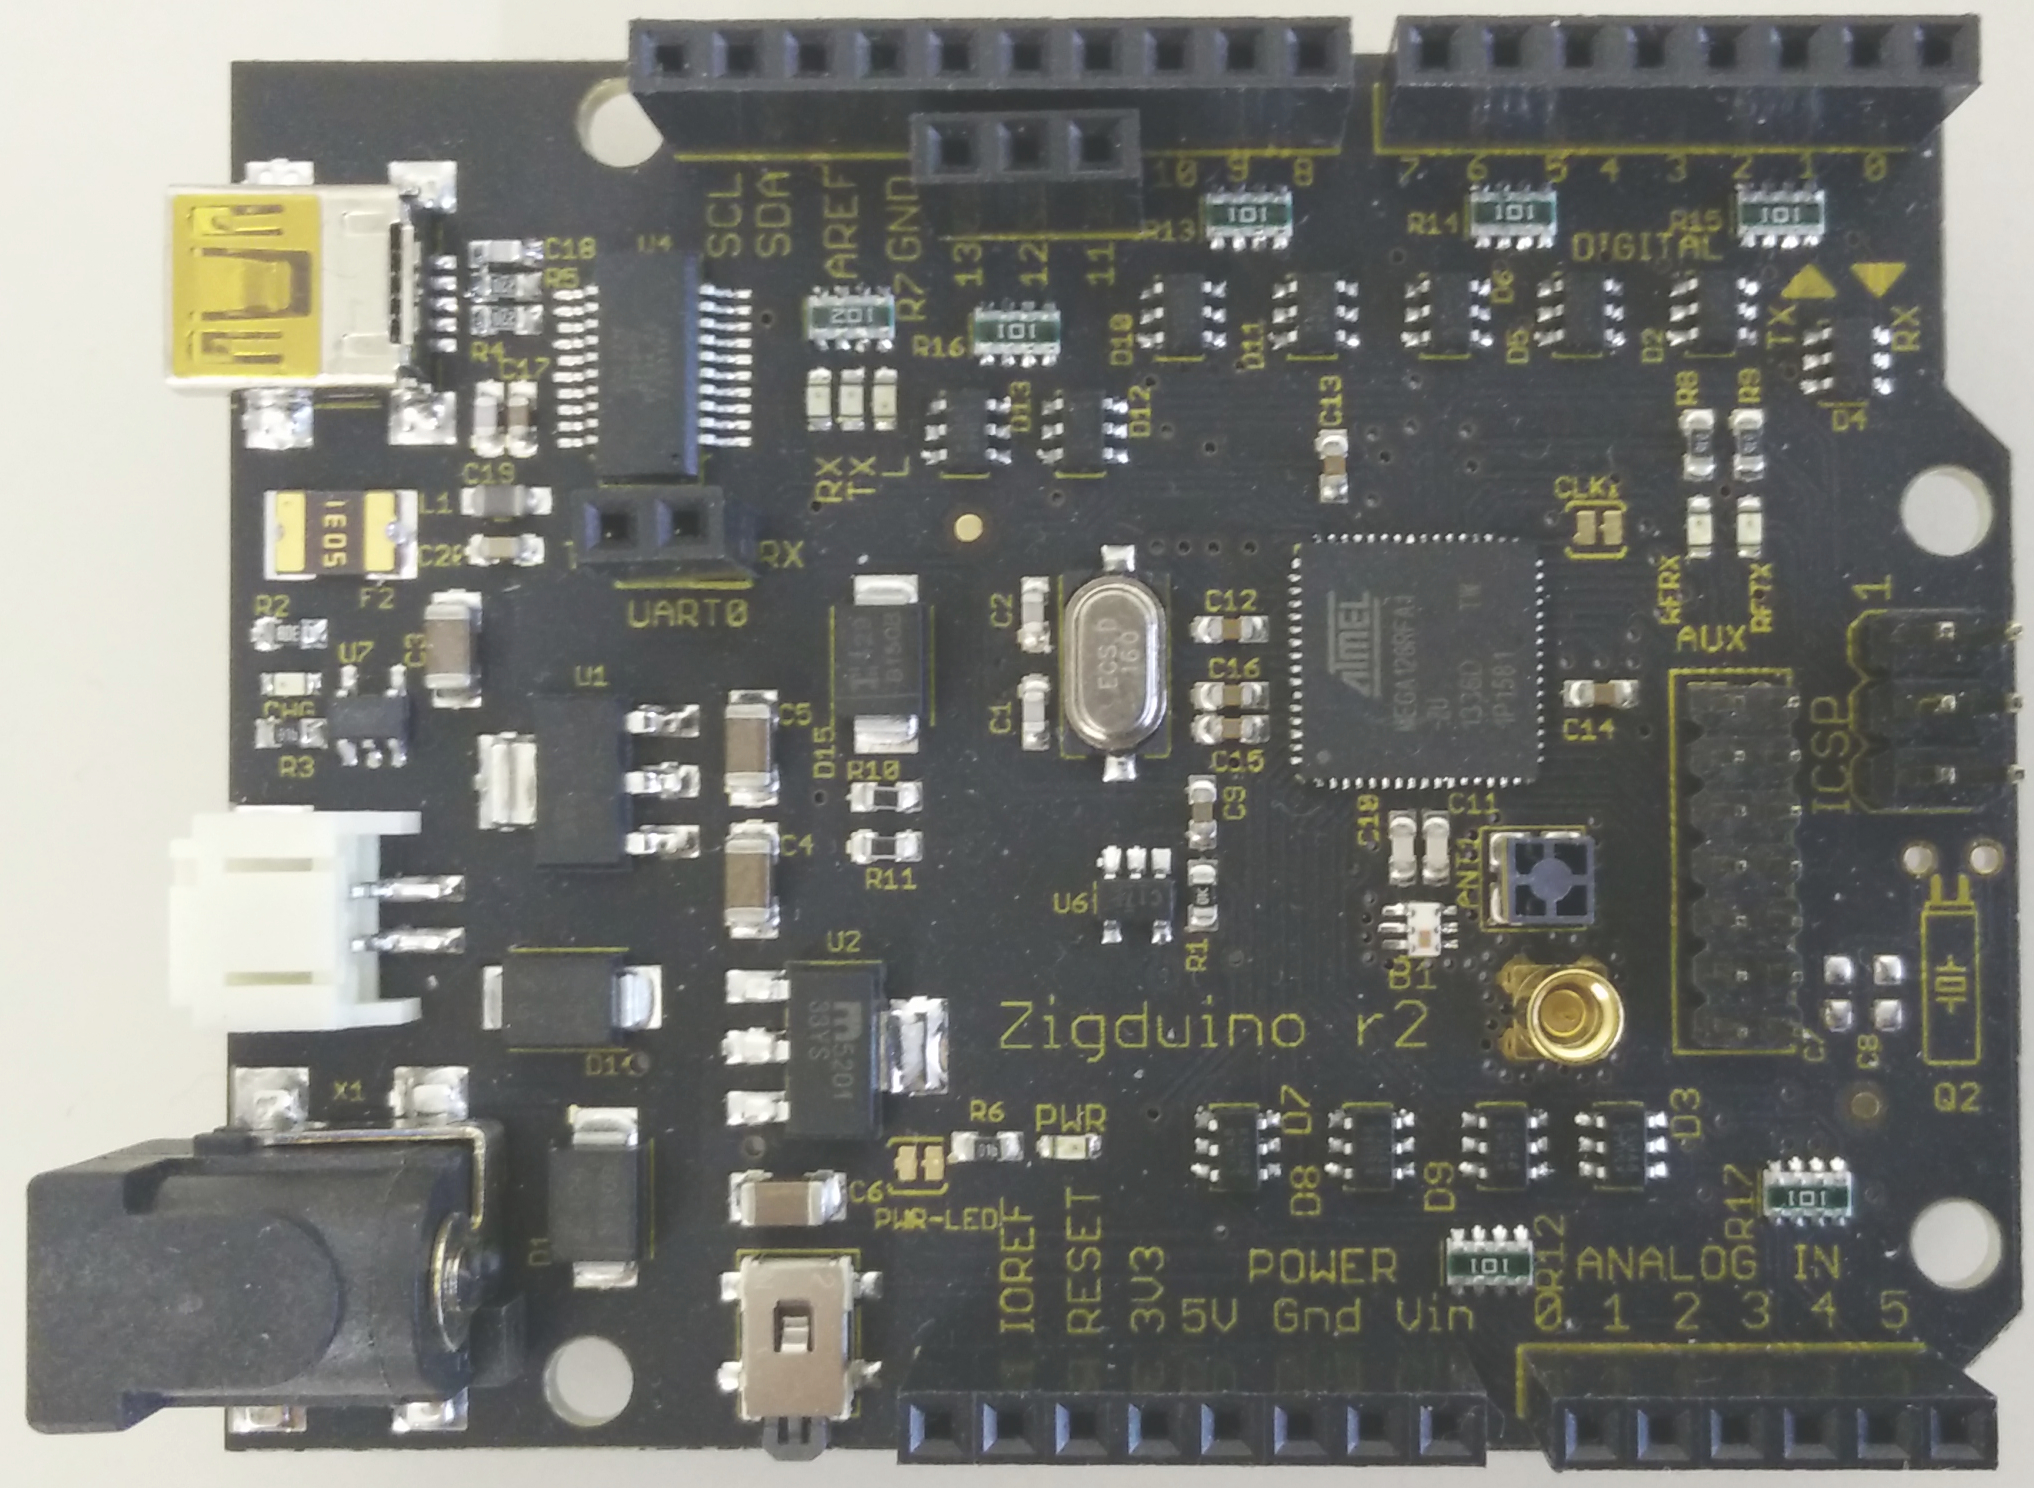
\includegraphics[height=0.78\textheight,keepaspectration=true]{zigduino.jpg}}
%     \caption{Een Zigduino}
%   \end{figure}
%   \note{
%   \begin{itemize}
%   \item embedded device
%   \item RF antenne, geen wifi, minder energie, groter bereik
%   \item sensoren worden aangesloten
%   \item microcontroller COMPUTEr ON A CHIP
%   \end{itemize}
% }
% \end{frame}

\begin{frame}{Wireless sensor networks}
  \begin{figure}
    \fbox{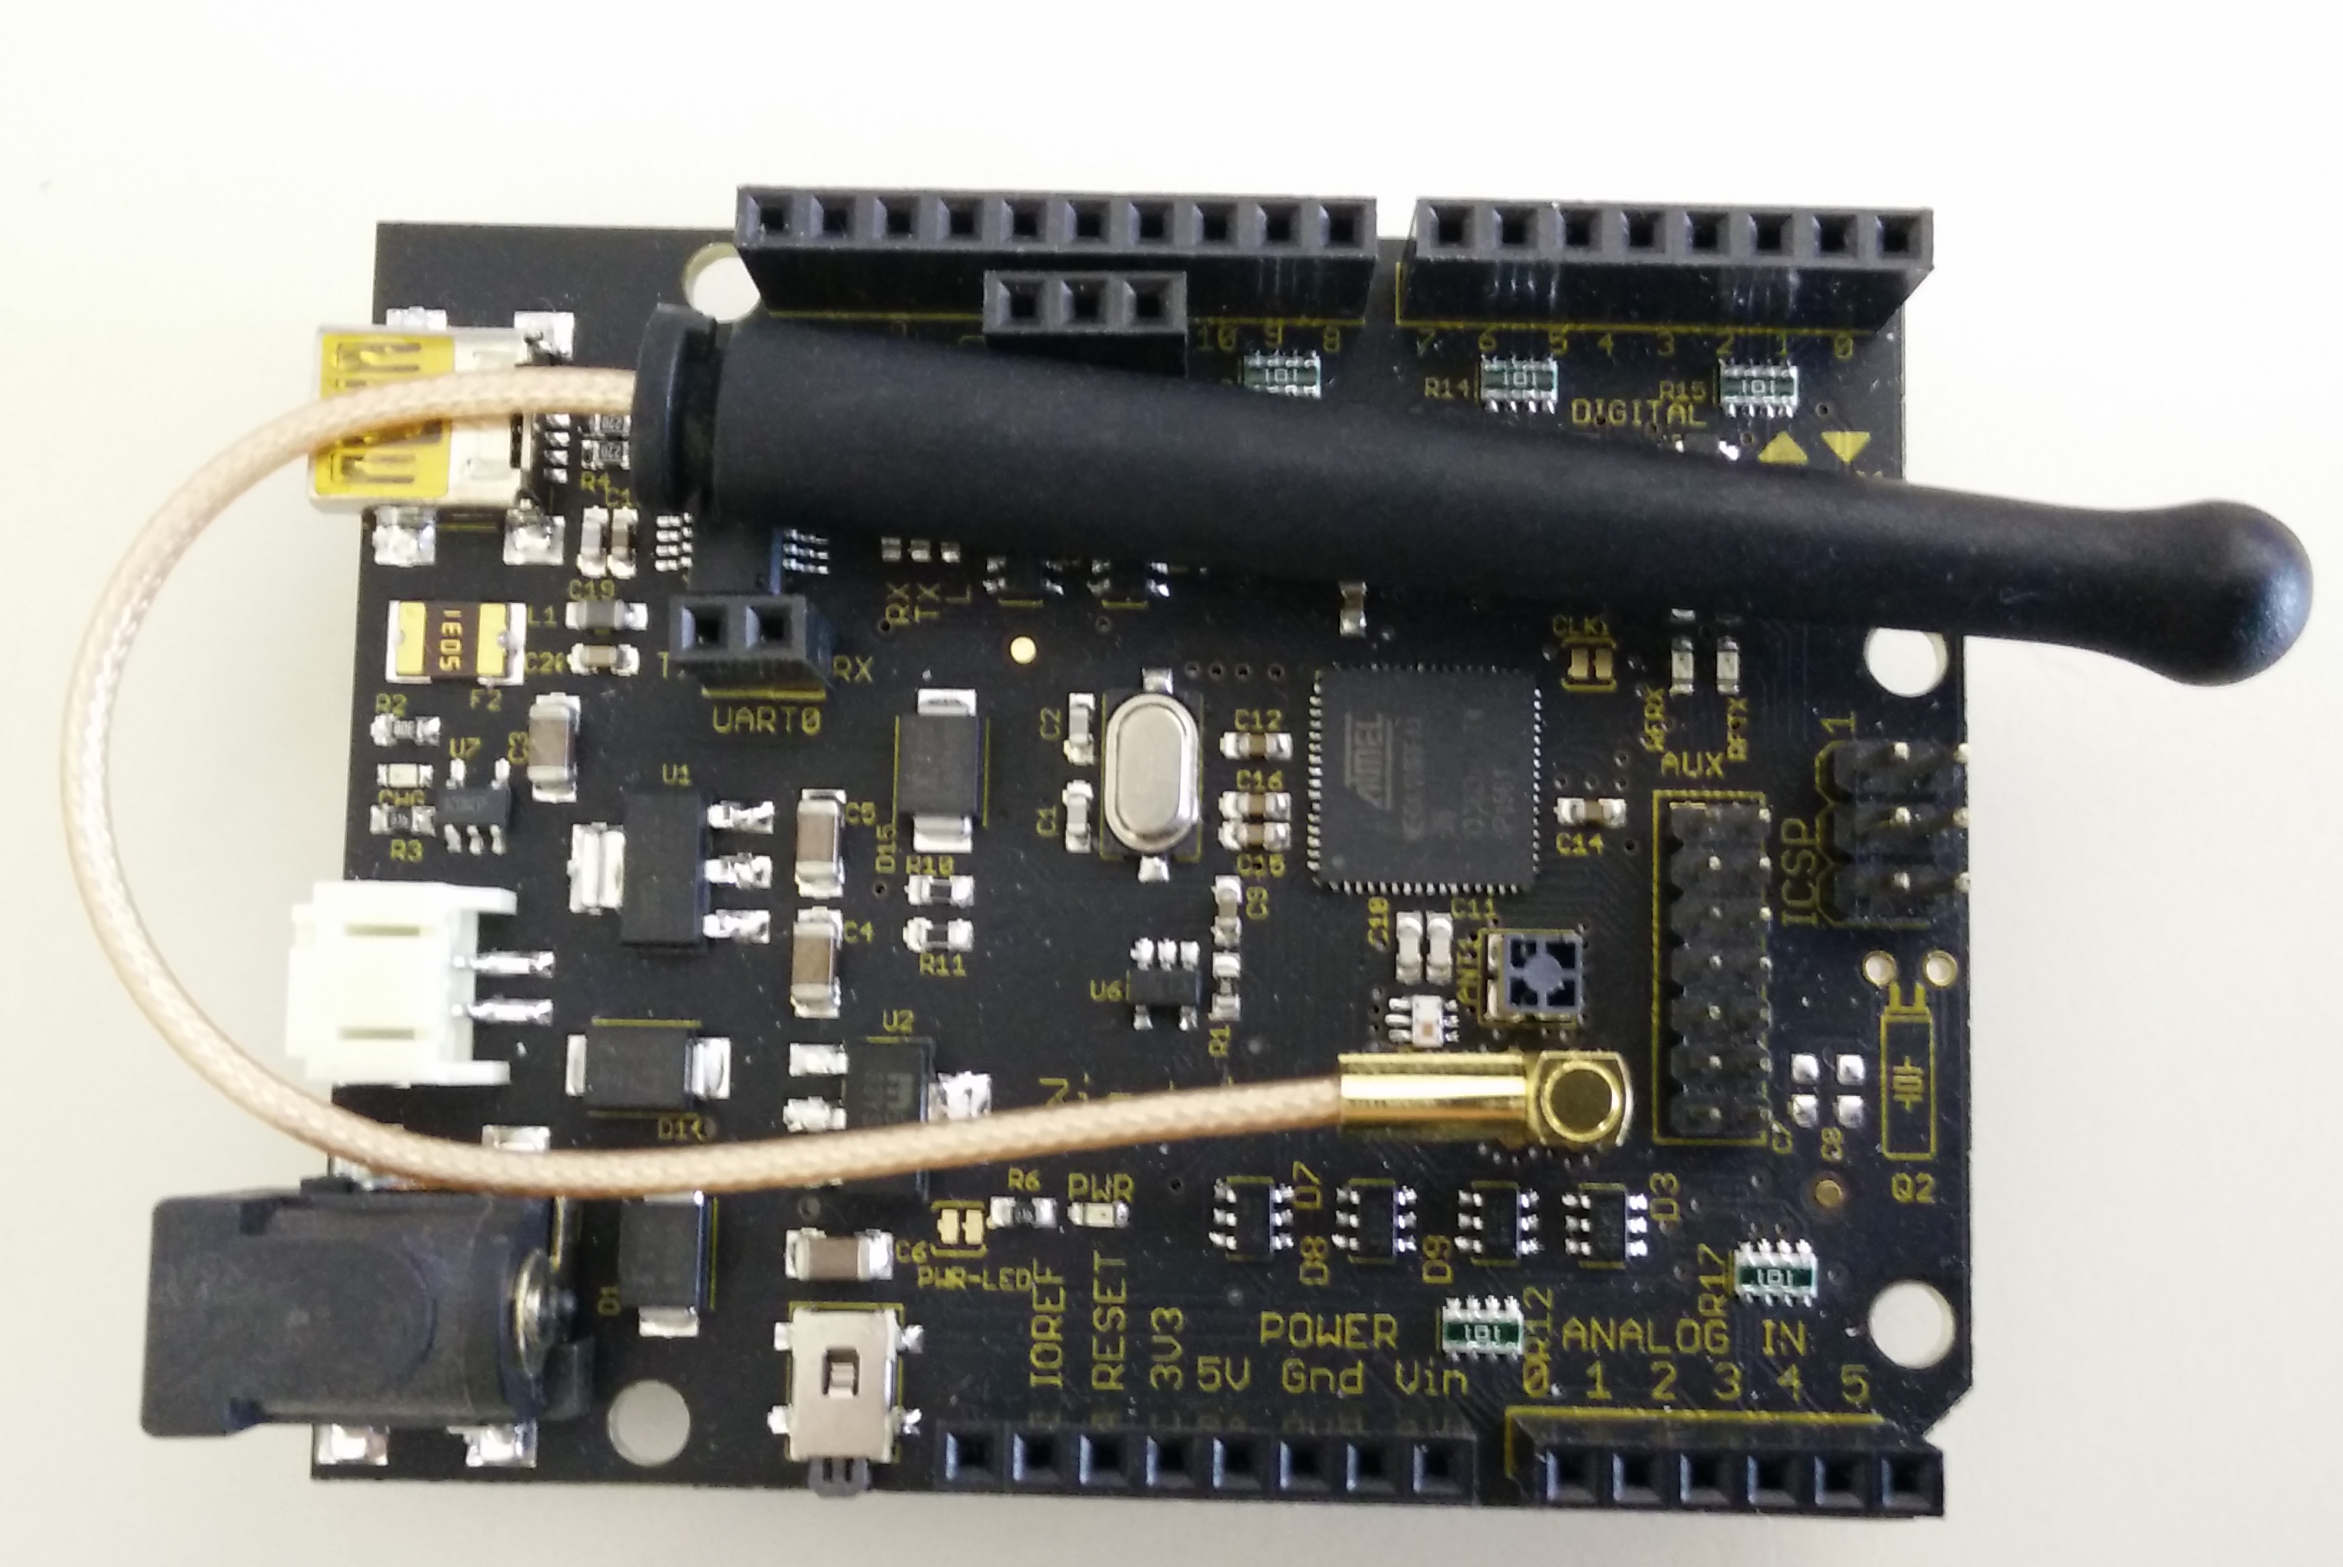
\includegraphics[height=0.78\textheight,keepaspectration=true]{zigduino_antenne.jpg}}
    \caption{Een Zigduino, met antenne}
  \end{figure}
  \note{
    \begin{itemize}
    \item embedded device
    \item RF antenne, geen wifi, minder energie, groter bereik
    \item sensoren worden aangesloten
    \item microcontroller COMPUTEr ON A CHIP
    \end{itemize}
  }
\end{frame}

\begin{frame}{Belangrijke aspecten bij WSN-design}
  \uncover<2->{\begin{block}{energie-effici\"ent}
      tot 10 jaar meegaan op \'e\'en batterij
    \end{block}}%
  \uncover<3->{\begin{block}{dichtheid}
      tot 20 sensor nodes per $m^3$ (geen harde limiet)
    \end{block}}%
  \uncover<4->{\begin{block}{goedkoop}
      \$1 of minder voor heel grootschalige deployments
    \end{block}}%
  \uncover<5->{\begin{block}{autonoom}
      deploy and forget
    \end{block}}%
  \uncover<6->{\begin{block}{adaptief}
      makkelijke aanpasbare topologie, bestand tegen falen van motes
    \end{block}}
  \note{
    \begin{itemize}
    \item energie efficeit tot 10 jaar
    \item dichtheid, zie geneeskunde
    \item grote hoeveelheid, dus moet goedkoop, moet kapot gaan
    \item autonoom deploy and forget
    \item adaptief, topologie verandert, falende motes
    \end{itemize}}
\end{frame}



\section{Probleemstelling}

\begin{frame}{Probleemstelling}
  \hiddencell{1}{	\large{Onze focus: \textbf{energie-efficiëntie}.}}
  \hiddencell{2}{
    \begin{exampleblock}{}
      {\textbf{Onderzoeksvraag:} Is het mogelijk om energie-efficiënter gegevens te verwerken door het te doen op een embedded IoT-toestel i.p.v. de back-end van het systeem?}
    \end{exampleblock}}

  \hiddencell{3}{
    \begin{center}

      \begin{tikzpicture}
        \filldraw[blue_kuleuven] (0,0) -- (5,0) -- (2.5,-1) -- (0,0);
        \node[text width=3cm] at (2.34,-0.25) {\textcolor{white}{Concretisering}};
      \end{tikzpicture}
      
    \end{center}
  }
  \begin{exampleblock}{}
    {\textbf{Onderzoeksopgave:} Vind een simpele \textit{metric} om snel te kunnen bepalen waar bepaalde code moet uitgevoerd worden.}
  \end{exampleblock}
\end{frame}

\section{Methodologie}
\begin{frame}{Methodologie}
  \large{Energie berekenen voor:}
  \vfill
  \begin{tabular}{c c c}
    \hiddencell{2}{
\includegraphics[width=0.25\textwidth,keepaspectration=true]{storage}} & \hiddencell{3}{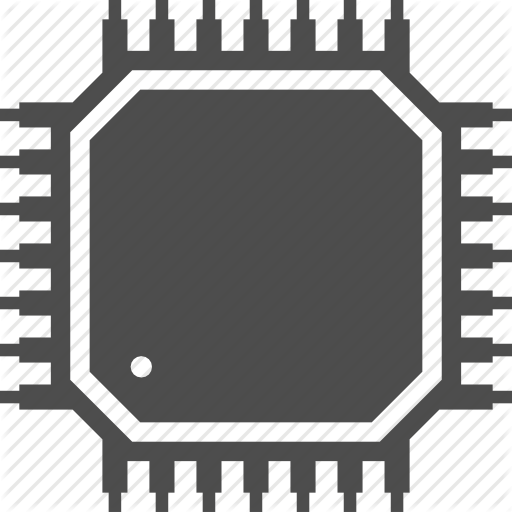
\includegraphics[width=0.25\textwidth,keepaspectration=true]{cpu}} & \hiddencell{4}{
\includegraphics[width=0.25\textwidth,keepaspectration=true]{radio}}  \\
    \hiddencell{2}{RAM-opslag} & \hiddencell{3}{berekeningen} & \hiddencell{4}{netwerkoverdracht}
  \end{tabular}
\end{frame}

\begin{frame}{Methodologie}
  
  \begin{tabular}{ p{0.3\textwidth}  p{0.6\textwidth}   }
    \toprule
    \multicolumn{1}{c}{RAM-opslag} &      \multicolumn{1}{c}{Gegevens}  \\ 
    \cmidrule(r){1-1}\cmidrule(lr){2-2}
    \raisebox{-\totalheight}{
\includegraphics[width=0.3\textwidth,keepaspectration=true]{storage}}
                                   & 
                                     \begin{itemize}
                                     \item  Data nog niet beschikbaar
                                       \hiddencell{2}{\item  Zelf experimenten uitvoeren}
                                     \end{itemize}
    \\ 
    
  \end{tabular}
  
\end{frame}

\begin{frame}{Methodologie}
  
  \begin{tabular}{ p{0.3\textwidth}  p{0.6\textwidth}   }
    \toprule
    \multicolumn{1}{c}{Berekeningen} &      \multicolumn{1}{c}{Gegevens}  \\ 
    \cmidrule(r){1-1}\cmidrule(lr){2-2}
    \raisebox{-\totalheight}{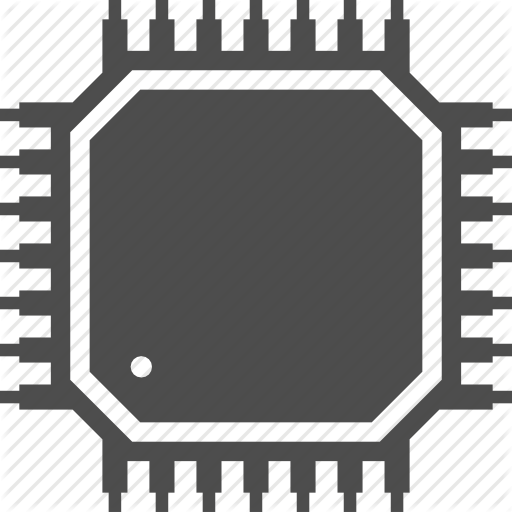
\includegraphics[width=0.3\textwidth,keepaspectration=true]{cpu}}
                                     & 
                                       \begin{itemize}
                                       \item  Data nog niet beschikbaar
                                         \hiddencell{2}{\item  Moeilijk te meten}
                                         \hiddencell{3}{\item  Theoretische aanpak}
                                       \end{itemize}
    \\ 
    
  \end{tabular}
  
\end{frame}

\begin{frame}{Methodologie}
  
  \begin{tabular}{ p{0.3\textwidth}  p{0.6\textwidth}   }
    \toprule
    \multicolumn{1}{c}{Antenne} &      \multicolumn{1}{c}{Gegevens}  \\ 
    \cmidrule(r){1-1}\cmidrule(lr){2-2}
    \raisebox{-\totalheight}
    {
\includegraphics[width=0.3\textwidth,keepaspectration=true]{radio}}
                                & 
                                  \begin{itemize}
                                  \item  Bestaat al deels data van
                                    \hiddencell{2}{\item  Ook moeilijk te meten}
                                    \hiddencell{3}{\item  Theoretische aanpak}
                                  \end{itemize}
    \\ 
    
  \end{tabular}
  
\end{frame}


\begin{frame}{Methodologie}
  \begin{figure}[center]
    \centering
    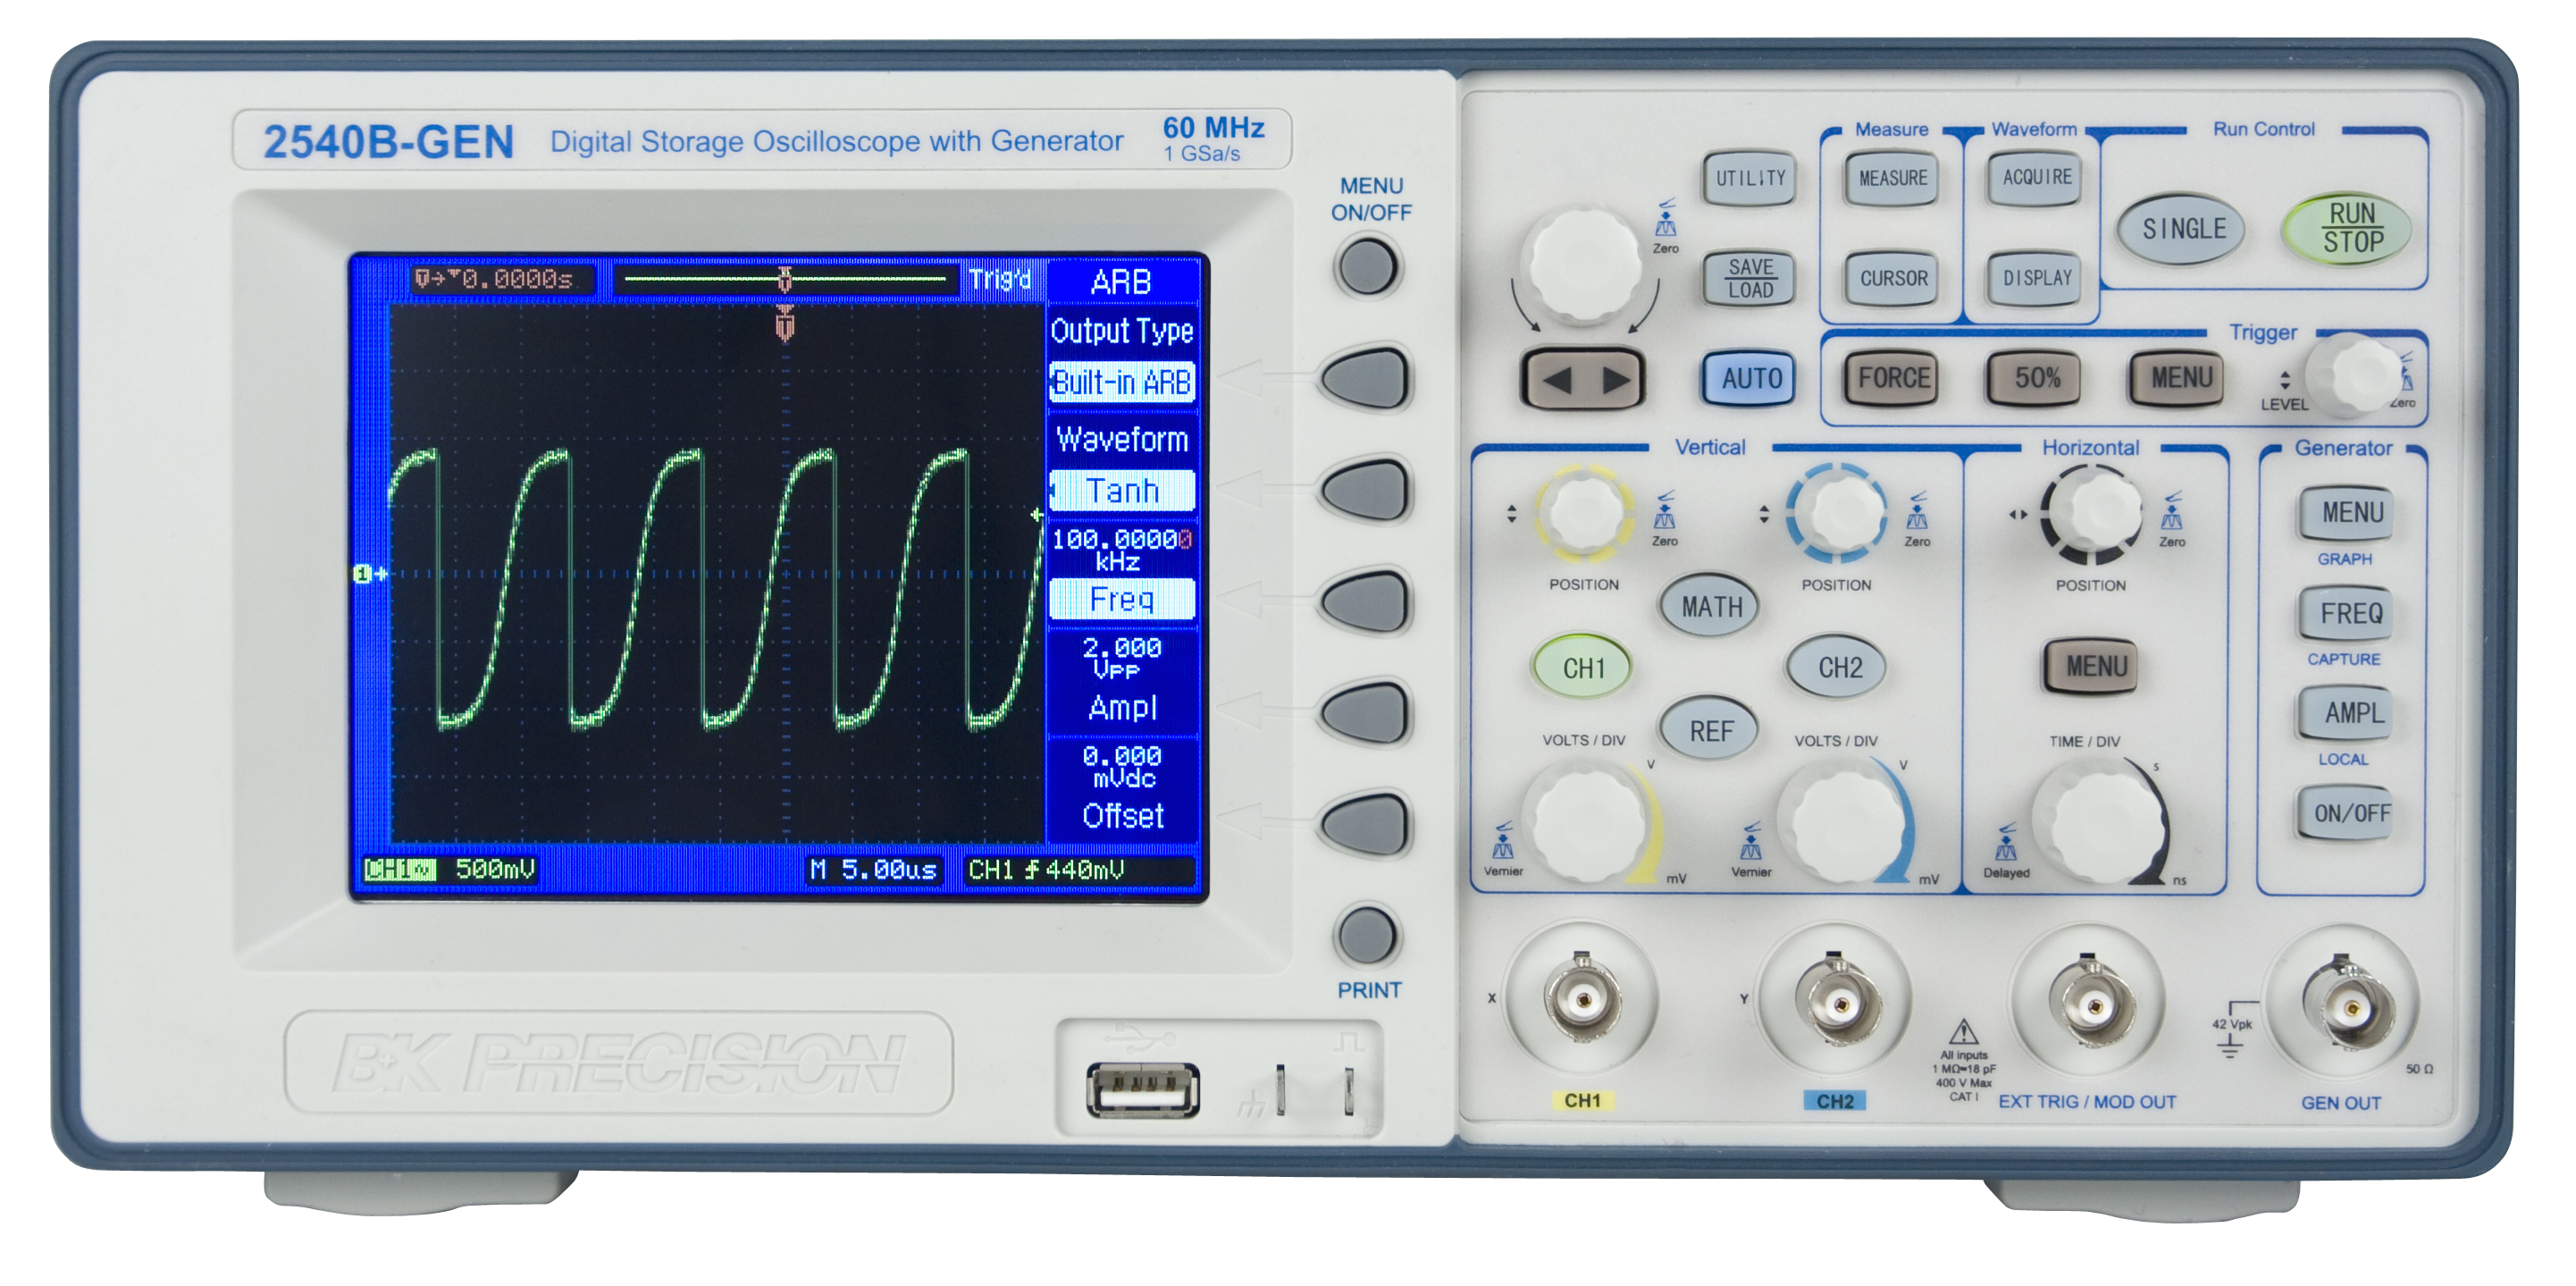
\includegraphics[width=0.9\textwidth,keepaspectration=true]{elek/dso}
    \caption{Oscilloscope}
  \end{figure}
\end{frame}

\begin{frame}{Methodologie}
  \begin{figure}[center]
    \centering
    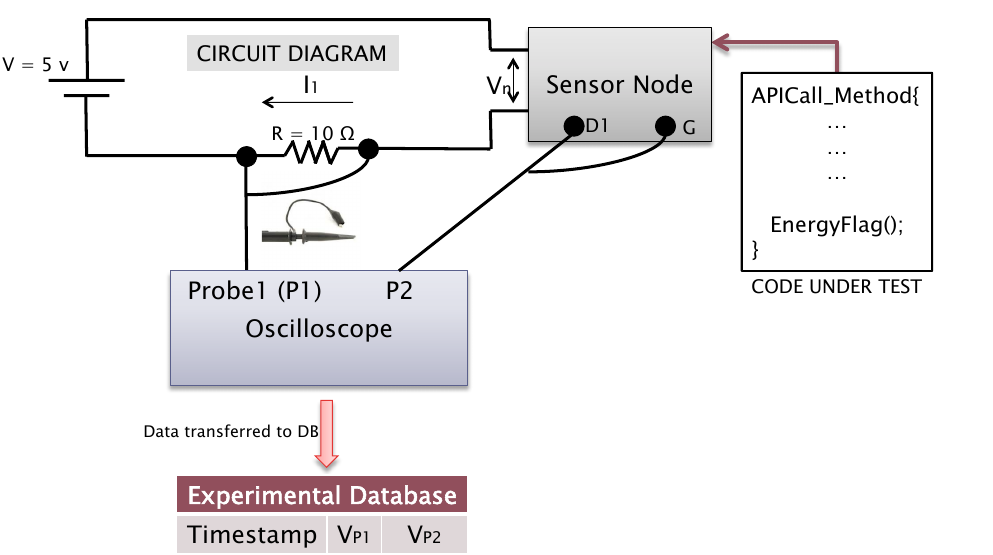
\includegraphics[width=0.9\textwidth,keepaspectration=true]{elek/diag1}
    \caption{Meetopstelling}
  \end{figure}
\end{frame}

% notes eigen foto gebruiken!!!
\begin{frame}{Methodologie}
  \begin{figure}[center]
    \centering
    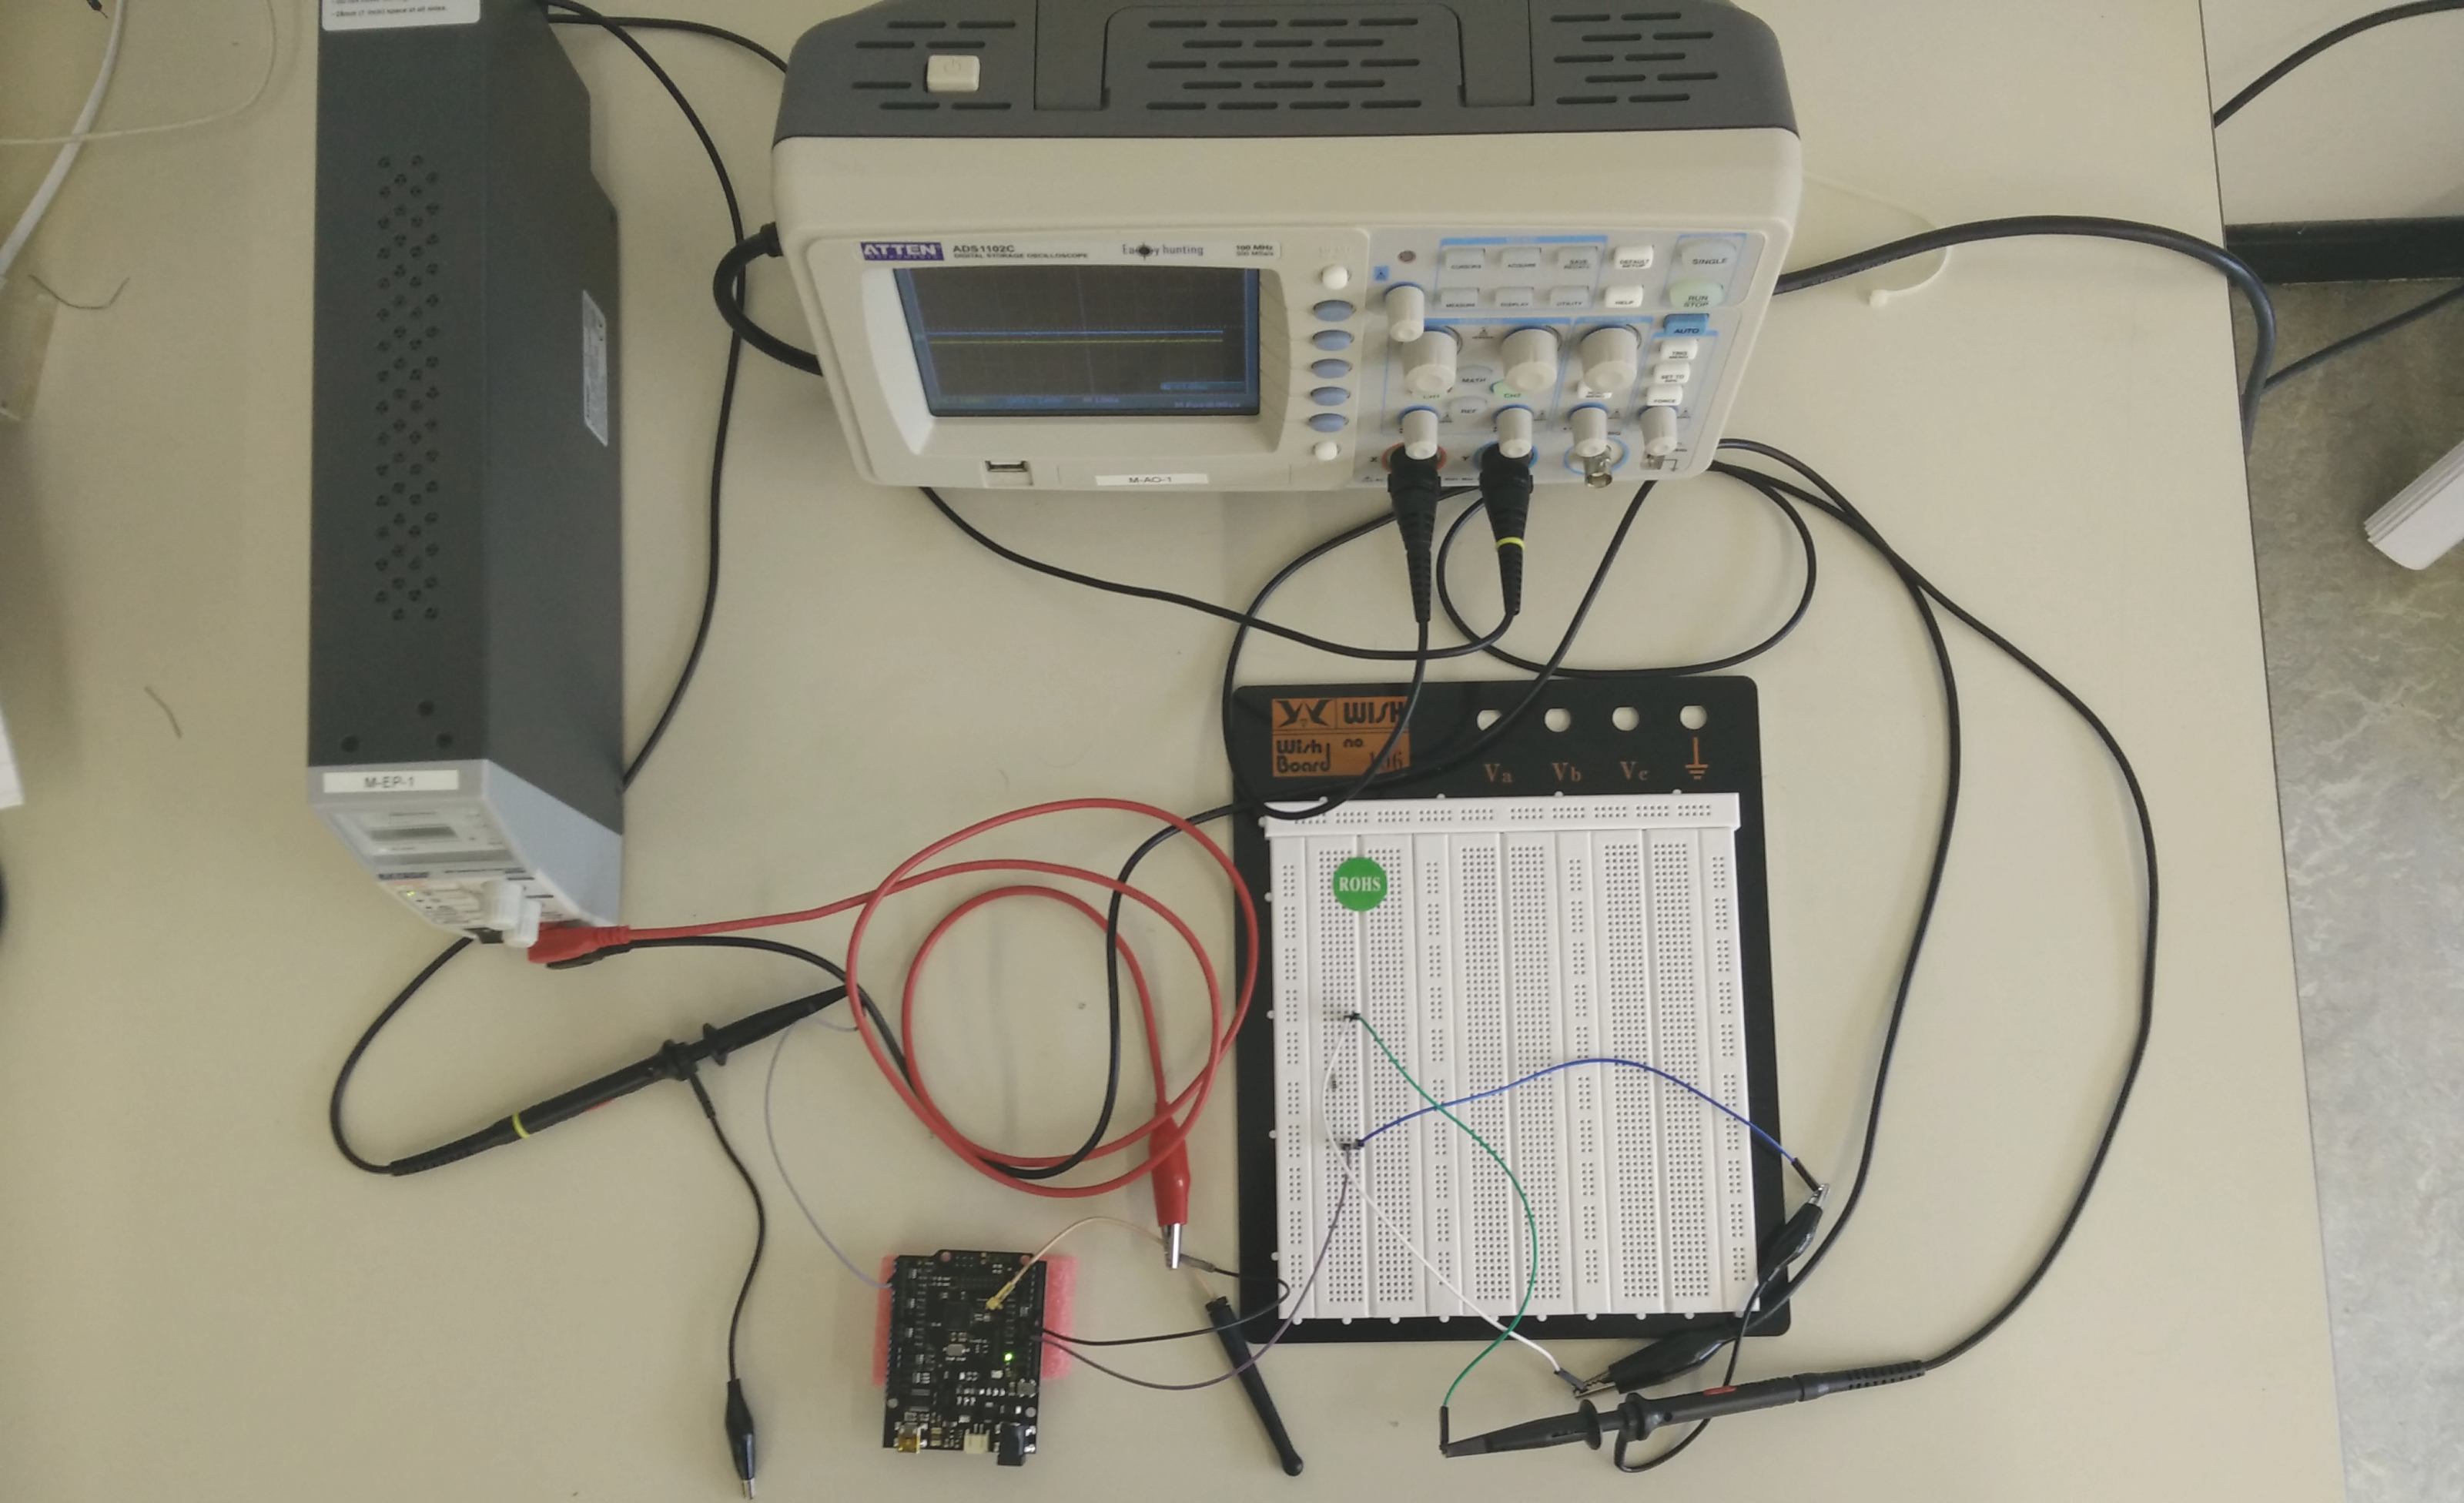
\includegraphics[width=0.9\textwidth,keepaspectration=true]{meetopstelling}
    \caption{Meetopstelling}
  \end{figure}
\end{frame}

\begin{frame}{Methodologie}
  
  \begin{tabular}{ p{0.47\textwidth}  p{0.47\textwidth}   }

    \begin{itemize}
    \item[] \textbf{1.} Maak component met triggers

    \end{itemize}
     & 

    \raisebox{-\totalheight}{
\includegraphics[width=0.4\textwidth,keepaspectration=true]{contiki}}\\

  \end{tabular}    
\end{frame}

\begin{frame}{Voorbeeld component}
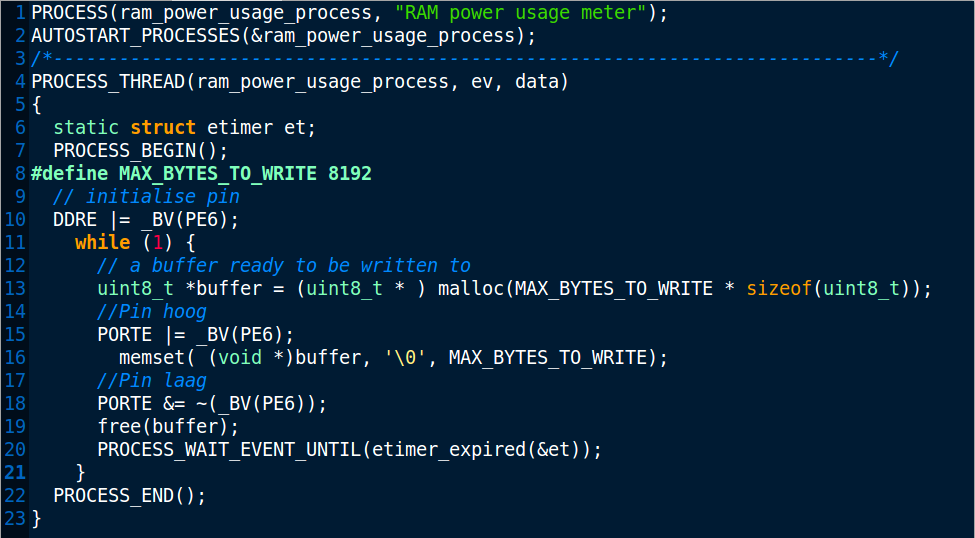
\includegraphics[width=0.99\textwidth,keepaspectration=true]{vbcode}
\end{frame}

\begin{frame}{Methodologie}
  
  \begin{tabular}{ p{0.47\textwidth}  p{0.47\textwidth}   }

    \begin{itemize}
    \item[] \textbf{1.} Maak component met triggers
    \item[] \textbf{2.} Laten uitvoeren
    \hiddencell{2}{\item[] \textbf{3.} Verwerk de data}
    \end{itemize}
    & 

    \raisebox{-\totalheight}{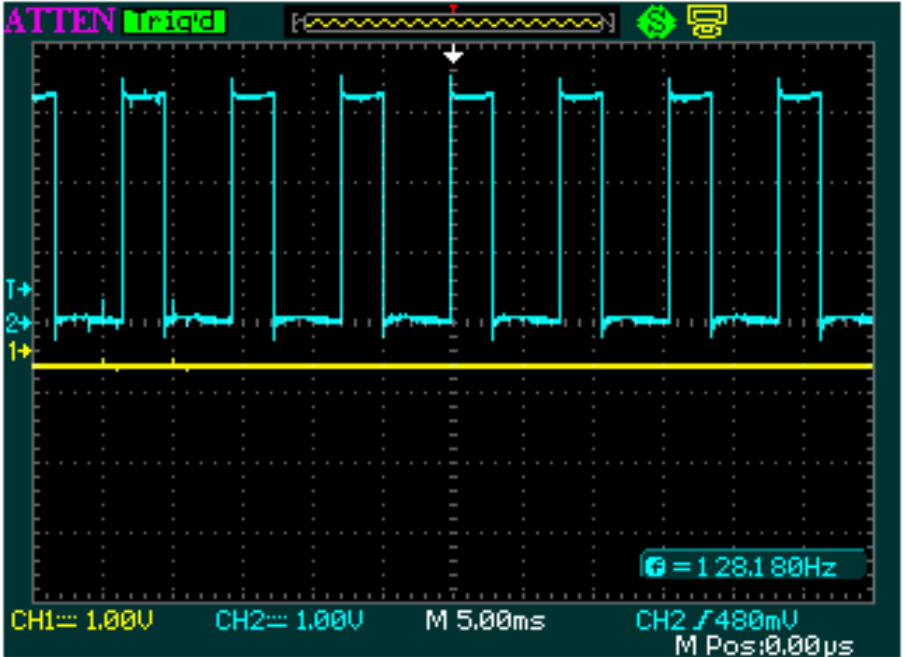
\includegraphics[width=0.4\textwidth,keepaspectration=true]{osc}}\\

  \end{tabular}    
\end{frame}

\begin{frame}{Voorbeeld data}
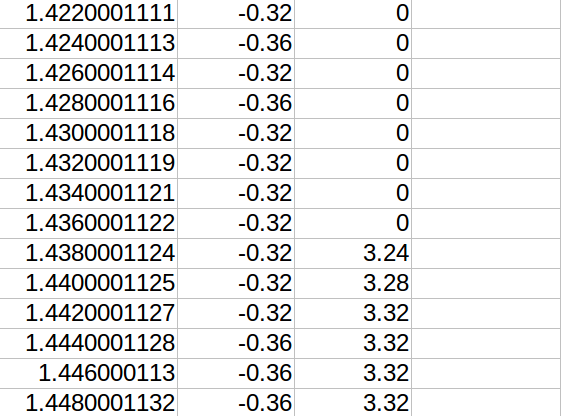
\includegraphics[width=0.99\textwidth,keepaspectration=true]{vbdata}
\end{frame}
%%%%%%%%%%%%%%%%%%%%%%%%%%%%%%%%%%%%%%%%%%%%%%%%%%%%%%%%%%%%%%%%%%%%%%%%%%%%%%%%% 

\begin{frame}{Methodologie}
  
  \begin{tabular}{ p{0.3\textwidth}  p{0.6\textwidth}   }
    \toprule
    \multicolumn{1}{c}{RAM-opslag} &      \multicolumn{1}{c}{Verwacht resultaat?}  \\ 
    \cmidrule(r){1-1}\cmidrule(lr){2-2}
    \raisebox{-\totalheight}{
\includegraphics[width=0.3\textwidth,keepaspectration=true]{storage}}
                                   & 
                                     \begin{itemize}
                                     \item Grootte: $16kB$
                                     \item Beschikbaar: $\pm 8kB$
                                     \item Verwachten een lineair verband
                                     \item Telkens groter aantal bytes schrijven
                                     \end{itemize}
    \\ 
    
  \end{tabular}
  
\end{frame}

\begin{frame}{Methodologie}
  
  \begin{tabular}{ c }
    \toprule
    \multicolumn{1}{c}{RAM-opslag}   \\ 
    \hline
    \raisebox{-\totalheight}{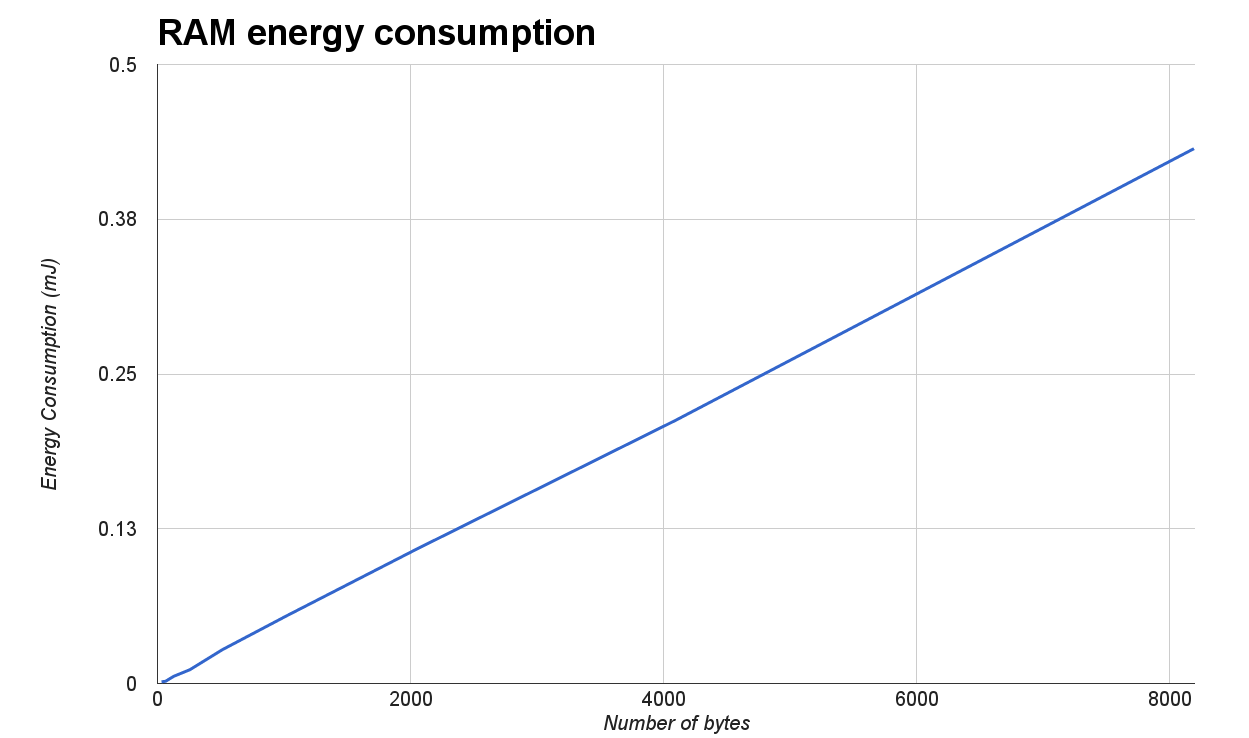
\includegraphics[width=0.95\textwidth,keepaspectration=true]{grafieken/ram_energie}}

    \\ 
    
  \end{tabular}
  
\end{frame}

\begin{frame}{Methodologie}
  
  \begin{tabular}{ p{0.25\textwidth}  p{0.7\textwidth}   }
    \toprule
    \multicolumn{1}{c}{RAM-opslag} &      \multicolumn{1}{c}{Resultaat}  \\ 
    \cmidrule(r){1-1}\cmidrule(lr){2-2}
    \raisebox{-\totalheight}{
\includegraphics[width=0.25\textwidth,keepaspectration=true]{storage}}
                                   & 
                                     \begin{itemize}
                                     \item  Grootte: $16kB$
                                     \item  Beschikbaar: $\pm 8kB$
                                     \item  Verwachten een lineair verband
                                     \item  Telkens groter aantal bytes schrijven
                                     \end{itemize}
                                     
                                     \framebox{\large{Lineair $\rightarrow 8.144\cdot 10^{-5}mJ/Byte$}}\\
  \end{tabular}
  
\end{frame}


%%%%%%%%%%%%%%%%%%%%%%%%%%%%%%%%%%%%%%%%%%%%%%%%%%%%%%%%%%%%%%%%%%%%%%%%%%%%%% 

\begin{frame}{Methodologie}
  
  \begin{tabular}{ p{0.3\textwidth}  p{0.6\textwidth}   }
    \toprule
    \multicolumn{1}{c}{berekeningen} &      \multicolumn{1}{c}{Verwacht resultaat?}  \\ 
    \cmidrule(r){1-1}\cmidrule(lr){2-2}
    \raisebox{-\totalheight}{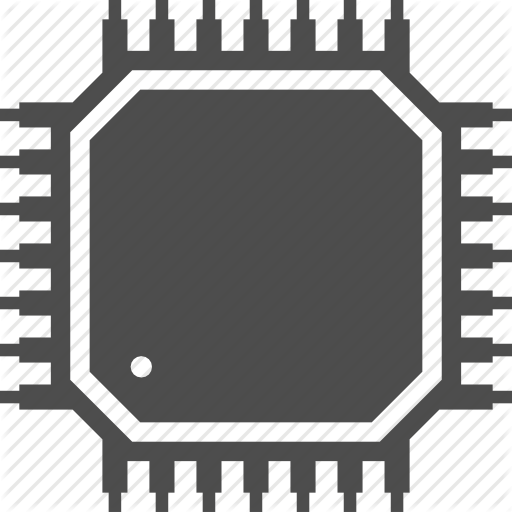
\includegraphics[width=0.3\textwidth,keepaspectration=true]{cpu}}
                                     & 
                                       \begin{itemize}
                                       \item  Opnieuw flags in code
                                       \item  Hiermee de tijd meten
                                       \item  Theoretische kost berekenen
                                       \item  Verwacht: kost verschilt van component tot component
                                       \end{itemize}
    \\ 
    
  \end{tabular}
  
\end{frame}

\begin{frame}{Methodologie}

  \begin{tabular}{ p{0.3\textwidth}  p{0.6\textwidth}   }
    \toprule
    \multicolumn{1}{c}{berekeningen} &      \multicolumn{1}{c}{Theretische berekening}  \\ 
    \cmidrule(r){1-1}\cmidrule(lr){2-2}
    \raisebox{-\totalheight}{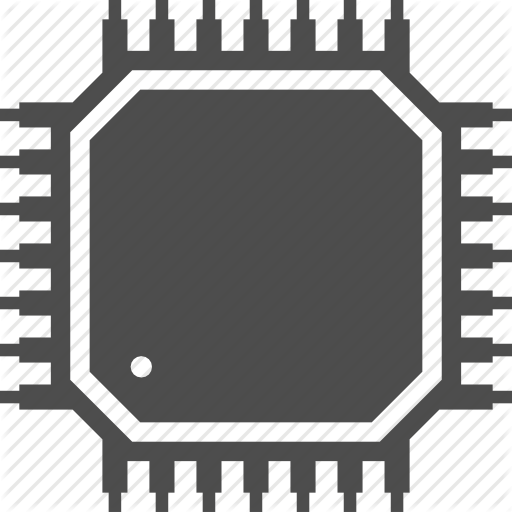
\includegraphics[width=0.3\textwidth,keepaspectration=true]{cpu}}
                                     & 
                                       \begin{itemize}
                                       \item  Tijd: $s$
                                       \item  Stroom: $3.7mA$
                                       \item  Voltage: $6V$
                                       \end{itemize}
                                       \framebox{Energie: $J = C \cdot V = A \cdot s \cdot V$ }
  \end{tabular}
  
\end{frame}

\begin{frame}{Methodologie}
  
  \begin{tabular}{ p{0.25\textwidth}  p{0.7\textwidth}   }
    \toprule
    \multicolumn{1}{c}{berekeningen} &      \multicolumn{1}{c}{Resultaat}  \\ 
    \cmidrule(r){1-1}\cmidrule(lr){2-2}
    \raisebox{-\totalheight}{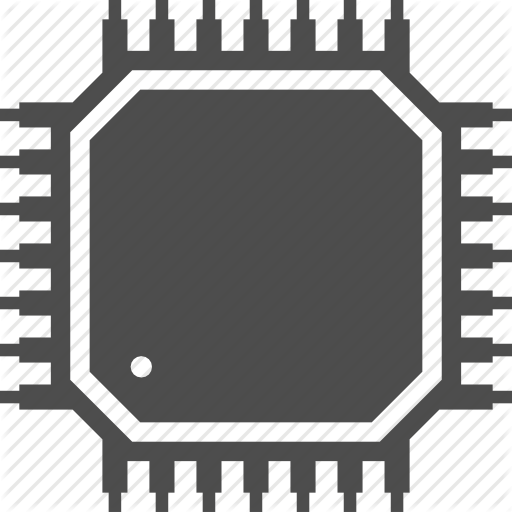
\includegraphics[width=0.25\textwidth,keepaspectration=true]{cpu}}
                                     & 
                                       \begin{itemize}
                                       \item  Tijd: $Nms$
                                       \item  Stroom: $3.7mA$
                                       \item  Voltage: $6V$
                                       \end{itemize}
                                       \framebox{Energie: $= 0.0037A \cdot Ns \cdot 6V$ }
  \end{tabular}
  
\end{frame}

%%%%%%%%%%%%%%%%%%%%%%%%%%%%%%%%%%%%%%%%%%%%%%%%%%%%%%%%%%%%%%%%%%%%%%%%%%%%%%%% 

\begin{frame}{Methodologie}
  
  \begin{tabular}{ p{0.3\textwidth}  p{0.6\textwidth}   }
    \toprule
    \multicolumn{1}{c}{Antenne} &      \multicolumn{1}{c}{Verwacht resultaat?}  \\ 
    \cmidrule(r){1-1}\cmidrule(lr){2-2}
    \raisebox{-\totalheight}{
\includegraphics[width=0.3\textwidth,keepaspectration=true]{radio}}
                                & 
                                  \begin{itemize}
                                  \item  Standaard RF-antenne
                                  \item  Vaste opstartkost
                                  \item  Daarna lineaire stijging (in functie van hoeveelheid bytes)
                                  \end{itemize}
    \\ 
    
  \end{tabular}
  
\end{frame}

\begin{frame}{Methodologie}
  
  \begin{tabular}{ p{0.3\textwidth}  p{0.6\textwidth}   }
    \toprule
    \multicolumn{1}{c}{Antenne} &      \multicolumn{1}{c}{Theoretische berekening}  \\ 
    \cmidrule(r){1-1}\cmidrule(lr){2-2}
    \raisebox{-\totalheight}{
\includegraphics[width=0.3\textwidth,keepaspectration=true]{radio}}
                                & 
                                  \begin{itemize}
                                  \item  Tijd: $s$
                                  \item  Hoeveelheid bytes: $N$ 
                                  \item  Constante opstarttijd: $113.104ms$
                                  \item  Tijdskost/byte: $0.382ms$
                                  \item  Stroom: $0.04A$
                                  \item  Voltage: $6V$
                                  \item  $J = C \cdot V = A \cdot s \cdot V$
                                  \end{itemize}
                                  
  \end{tabular}
  \begin{center}
    \framebox{Energie $= 0.04A \cdot (N \cdot 0.382 + 113.104)ms \cdot 6V$ }      
  \end{center}
\end{frame}




\begin{frame}{Methodologie}
  \begin{tabular}{ p{0.3\textwidth}  p{0.3\textwidth} p{0.3\textwidth}}
    \toprule
    & \multicolumn{1}{c}{Overzicht}  & \\ 
    \toprule
    RAM-opslag & berekeningen & Antenne\\
    \cmidrule(r){1-1}\cmidrule(lr){2-2}\cmidrule(l){3-3}
  \end{tabular}      
  \begin{minipage}{.33\textwidth}
    \centering
    Variabele: \# bytes\\
    \vspace{0.25cm}
    \fbox{$8.144\cdot 10^{-5}mJ/Byte$} 
    
  \end{minipage}%
  \begin{minipage}{.33\textwidth}
    \centering
    Variabele N: tijdsduur\\
    \vspace{0.25cm}
    \fbox{$0.0037A \cdot Nms \cdot 6V$}
    
  \end{minipage}
  \begin{minipage}{.3\textwidth}
    \centering
    Variabele N: bytes\\
    \vspace{0.35cm}
    \fbox{\parbox{\textwidth}{$0.04A \cdot (N \cdot 0.382$ \\ $+ 113.104)ms \cdot 6V$}}
    
  \end{minipage}
  \hiddencell{2}{
    \begin{tabular}{ p{0.3\textwidth}  p{0.3\textwidth} p{0.3\textwidth}}
      \hline
      & \multicolumn{1}{c}{Grootteorde voor 1ms:}  & \\ 
      \hline
    \end{tabular}  
  }
  \begin{minipage}{.33\textwidth}
    \hiddencell{3}{
      \vspace{0.25cm}
      \centering
      $\pm 3000$ bytes schrijven\\
      $\Rightarrow 0.2443 mJ$}
    
  \end{minipage}%
  \begin{minipage}{.33\textwidth}
    \hiddencell{4}{
      \centering
      $\Rightarrow 0.0222 mJ$}
    
  \end{minipage}
  \begin{minipage}{.3\textwidth}
    \hiddencell{5}{
      \vspace{0.25cm}
      \centering
      Opstartkost alleen:\\
      $\Rightarrow 27.14 mJ$}
    
  \end{minipage}
  
\end{frame}
%%%%%%%%%%%%%%%%%%%%%%%%%%%%%%%%%%%%%%%%%%%%%%%%%%%%%%%%%%%%%%%%%%%%%%%%%%%%%%%% 
%%%%%%%%%%%%%%%%%%%%%%%%%%%%%%%%%%%%%%%%%%%%%%%%%%%%%%%%%%%%%%%%%%%%%%%%%%%%%%%% 
%%%%%%%%%%%%%%%%%%%%%%%%%%%%%%%%%%%%%%%%%%%%%%%%%%%%%%%%%%%%%%%%%%%%%%%%%%%%%%%% 
%%%%%%%%%%%%%%%%%%%%%%%%%%%%%%%%%%%%%%%%%%%%%%%%%%%%%%%%%%%%%%%%%%%%%%%%%%%%%%%% 
%%%%%%%%%%%%%%%%%%%%%%%%%%%%%%%%%%%%%%%%%%%%%%%%%%%%%%%%%%%%%%%%%%%%%%%%%%%%%%%% 
%%%%%%%%%%%%%%%%%%%%%%%%%%%%%%%%%%%%%%%%%%%%%%%%%%%%%%%%%%%%%%%%%%%%%%%%%%%%%%%% 
%%%%%%%%%%%%%%%%%%%%%%%%%%%%%%%%%%%%%%%%%%%%%%%%%%%%%%%%%%%%%%%%%%%%%%%%%%%%%%%% 
%%%%%%%%%%%%%%%%%%%%%%%%%%%%%%%%%%%%%%%%%%%%%%%%%%%%%%%%%%%%%%%%%%%%%%%%%%%%%%%% 
\section{Voorgestelde oplossing}

\begin{frame}{Voorgestelde oplossing}
  Wat weten we tot nu toe?
  \begin{itemize}
  \item RAM: zo goed als gratis.
    \hiddencell{2}{\item CPU: relatief goedkoop.}
    \hiddencell{3}{\item Antenne: zeer duur $\rightarrow$ hoge opstartkost.}

  \end{itemize}

  \hiddencell{4}{$\Rightarrow$ Gebruik CPU en RAM om data te reduceren}

\end{frame}

\begin{frame}{Voorgestelde oplossing}
  % TODO XAVIER: onze metric in een mooie formule gieten
  \begin{equation}
    \begin{split}
      h : x \mapsto \{0, 1\} \\
      h(x) = signum(transmit(x) - cost(reduce(x)) \\ - cost(transmit(reduce(x))))
    \end{split}

\[
    h(x)= 
\begin{cases}
  1, & \text{als } transmit(x) - cost(reduce(x)) - cost(transmit(reduce(x)))  \\
  0, & \text{otherwise}
\end{cases}
\]

  \end{equation}

\end{frame}

\section{Resultaten}
% TODO betere naam omgevins...
\begin{frame}{Toetsen aan praktijkscenario's}

  \begin{enumerate}
  \item Temperatuurmeting
  \item Omgevingsaangenaamheid
  \end{enumerate}
\end{frame}

\begin{frame}{Temperatuur meting}

\end{frame}

\begin{frame}{Temperatuur meting}

\end{frame}

\begin{frame}{Omgevingsaangenaamheid}
  Verschillende sensoren combineren om aangenaamheid te bepalen:
  \begin{itemize}
	\item Temperatuur, Vochtigheid, Geluid
	\item Elke meting 2 bytes
	\item Totaal 6 bytes
	\item Aangenaam indien elke sensorwaarde in bepaald interval ligt.
  \end{itemize}


\end{frame}

\begin{frame}{Omgevingsaangenaamheid}
  Reduceren we op basis van hoeveelheid data die we doorsturen\\
  Bereken op de mote of aangenaam is:
  \begin{itemize}
    \hiddencell{2}{\item Reductie: $6n \mapsto n$}
    \hiddencell{3}{\item CPU: 3x 2 vergelijkingen $\rightarrow \pm$ gratis}
    \hiddencell{4}{\item RAM: niet meer als bij S\& S.}
  \end{itemize}

\end{frame}

\begin{frame}{Omgevingsaangenaamheid: resultaat}
  Bereken op de mote of aangenaam is:
  \begin{itemize}
	\item Reductie: $6n \mapsto n$
	\item CPU: 3x 2 vergelijking $\rightarrow \pm$ gratis
	\item RAM: niet meer als bij S\& S.
  \end{itemize}
  $\Rightarrow$ even nauwkeurig maar 6x minder data verzenden!

\end{frame}

\section{Een kort scenario: temperatuurmetingen}

\begin{frame}{Setup}
  \begin{itemize}
  \item taak: observeer de temperatuur
  \item 
  \end{itemize}
\end{frame}

\begin{frame}{Strategie\"en}
  \begin{itemize}
  \item sense and send
  \item filter
  \item aggregate
  \item average
  \end{itemize}
\end{frame}

\begin{frame}{Demo}
  \begin{center}
    \Huge{DEMO}
  \end{center}

\end{frame}

\begin{frame}{Demo}
  \begin{center}
    \Huge{DEMO}
  \end{center}

\end{frame}

\section{Conclusie \& verder werk}
\begin{frame}{Conclusie}
  2 grote categoriën:
  \vspace{1cm}
  \begin{tabular}{ p{5.5cm}  p{5.5cm} }
    \toprule
    Reductie doorstuurfrequentie & Reductie doorstuurhoeveelheid   \\ 
    \toprule
  \end{tabular}    

  \begin{minipage}{.5\textwidth}
    \begin{itemize}
    \item Zeer efficiënt
    \item Minder naukeurig
    \item Gemakkelijker te implementeren
    \end{itemize}
    
  \end{minipage}%
  \begin{minipage}{.5\textwidth}
    \begin{itemize}
    \item Behoudt naukeurigheid
    \item Moeilijker te ïmplementeren
    \item Minder efficiënt
    \end{itemize}
  \end{minipage}
  \vspace{2cm}
  \hspace{2.5cm}
  \fbox{$\Rightarrow$ maak een combinatie}
\end{frame}

\begin{frame}{Verder werk}
  \begin{itemize}
  \item Reductie uitwerken over volledige topologieën van netwerken.
  \item Optimale reductie vinden.
    % TODO plot van xavier?
  \end{itemize}
\end{frame}

%%%%%%%%%%%%%%%%%%%%%%%%%%%%%%%%%%%%%%%%%%%%%%%%%%%%%%%%%%%%%%% 
\begin{frame}[allowframebreaks]{Bibliografie}

  % \addtocategory{papers}{akyildiz2002wireless}
  % \addtocategory{papers}{mainwaring2002wireless}
  % \addtocategory{papers}{hughes2009looci}
  % \addtocategory{papers}{hughes2013energy}
  \nocite{*}
  % \textbf{Papers}
  % \printbibliography[category=papers]
  % \newpage
  % \textbf{Afbeeldingen}
  % \printbibliography[type=misc]
  \printbibliography
\end{frame}

\end{document}
